\documentclass{article}

\usepackage{rebuttal/rebuttal}

\usepackage[utf8]{inputenc} % allow utf-8 input
\usepackage[T1]{fontenc}    % use 8-bit T1 fonts
\usepackage{hyperref}       % hyperlinks
\usepackage{url}            % simple URL typesetting
\usepackage{booktabs}       % professional-quality tables
\usepackage{amsfonts}       % blackboard math symbols
\usepackage{nicefrac}       % compact symbols for 1/2, etc.
\usepackage{microtype}      % microtypography
\usepackage{graphicx}
\usepackage{xcolor}
\usepackage{float}
\usepackage{wrapfig}
\usepackage{amsthm}
\usepackage{amsmath} % provides many mathematical environments & tools
\usepackage{dsfont}
\usepackage{subcaption}
\usepackage{xspace}

\usepackage{lipsum}

\definecolor{cl5}{rgb}{1,0.73,0}
\definecolor{cl6}{rgb}{0,0.63,1}
\definecolor{cl2}{rgb}{0.4,0,1.0}
\definecolor{cl3}{rgb}{0,0.8,1}
\definecolor{cl4}{rgb}{1,0,0.6}
\definecolor{cl1}{rgb}{0.93,0.64, 0.06}
\definecolor{cl7}{rgb}{1,0.83, 0}
\definecolor{cl8}{rgb}{0.1,0.48, 0.11}
\definecolor{cl9}{rgb}{0.65,0.15, 0.15}
\definecolor{cl10}{rgb}{0.5,0.5, 1.0}
\definecolor{cl11}{rgb}{0.5,0.5,0.5}

\newcommand{\hl}[1]{\textbf{\textcolor{cl9}{#1}}}
\newcommand{\qu}[1]{\textit{#1}}

\newcommand{\ac}{SupSup\xspace}
\newcommand{\casename}[1]{\ensuremath{\mathsf{#1}}\xspace}

%\newcommand{\rone}{\textbf{\textbf{\textcolor{cl7}{R1}}}}
%\newcommand{\rtwo}{\textbf{\textbf{\textcolor{cl11}{R2}}}}
%\newcommand{\rthree}{\textbf{\textbf{\textcolor{cl10}{R3}}}}

\newcommand{\rone}{\textbf{\textcolor{cl11}{R1}}}
\newcommand{\rtwo}{\textbf{{\textcolor{cl6}{R2}}}}
\newcommand{\rthree}{\textbf{{\textcolor{cl10}{R3}}}}
\newcommand{\todo}[1]{\comments{\textcolor{red}{[TODO: #1]}}}

\begin{document}

% $\rone$ mentions that this work \qu{explores an important direction in NAS}. $\rtwo$ mentions that this work provides \qu{an especially elegant description of the network design problem ... the unification of core parts of the sparse neural network literature combined with the neural architecture search problem is very nice, and will mean that the paper of interest to a very large cross-section of the NeurIPS community}. $\rthree$ mentions that the paper \qu{has a strong significance, as it studies the still poorly explored venue of learning good connection patterns for neural networks}. 
\noindent \textbf{\textcolor{cl11}{\textbullet}} $\rone$: Thank you for the great suggestions and thorough review, we look forward to fully incorporating your detailed recommendations to improve the paper.

\textbf{Empirical comparison between binary and one-shot.} An empirical comparison between the binary and one-shot algorithms is a fantastic addition: In Figure 1 \textbf{(left)} we directly interpolate between these two algorithms. We replace line 6 of the binary algorithm, $g_i \leq {\textbf{median}(g)}$, with $g_i \leq {\textbf{top-}\gamma\%\textbf{-element}(g)}$. Then when $\gamma=1/2$ we recover the binary algorithm (as $\textbf{median}(g) = \textbf{top-}50\%\textbf{-element}(g)$) and when $\gamma=1/k$ we recover the one-shot algorithm. A performance drop is observed from binary to one-shot for the difficult task of MNISTRotate---sequentially learning 36 rotations of MNIST (each new rotation differing by only 10 degrees).

\textbf{Further comparison in \casename{GNu}.} We believe the comparison of SupSup (in \casename{GNu}) with recent methods (PSP [1], BatchE [2]) in the \casename{GG} scenario is fair since \casename{GG} is strictly easier than \casename{GNu}. However we agree that this is a weakness and will update the paper to compare SupSup with methods \textit{e.g.} from [3]. The initial reason for comparison of SupSup in \casename{GNu} with recent methods in the strictly easier \casename{GG} scenario is because they were more competitive. For instance [3] considers sequential learning problems with only 5-10 tasks. SupSup, after sequentially learning 250 permutations of MNIST, outperforms all non-replay methods from [3] in the \casename{GNu} scenario after they have learned only 10 permutations of MNIST with a similar network: In \casename{GNu}, Online EWC achieves 33.88\% \& SI achieves 29.31\% on 10 permutations of MNIST [3] while SupSup achieves 94.91\% accuracy after 250 permutations (see Table 5 in [3] vs. Table 7 in our work). 


\textbf{Additional comments.} We have updated the appendix to explicitly detail the supermask training algorithm, which improves clarity. The method provided for \casename{NNs} will not work with data that is common between tasks. We say that 16 bit integers are used instead of single bits because they store the index of the nonzero elements of the mask with the CSC sparse matrix format. PSP on SplitCIFAR achieves worse performance than BatchE (\casename{GG}) with similar bytes. We will definitely think about extensions of SupSup to the continuous case, but do not currently have a solution. 

\begin{figure}
    \begin{subfigure}{0.33\textwidth}
    \centering
    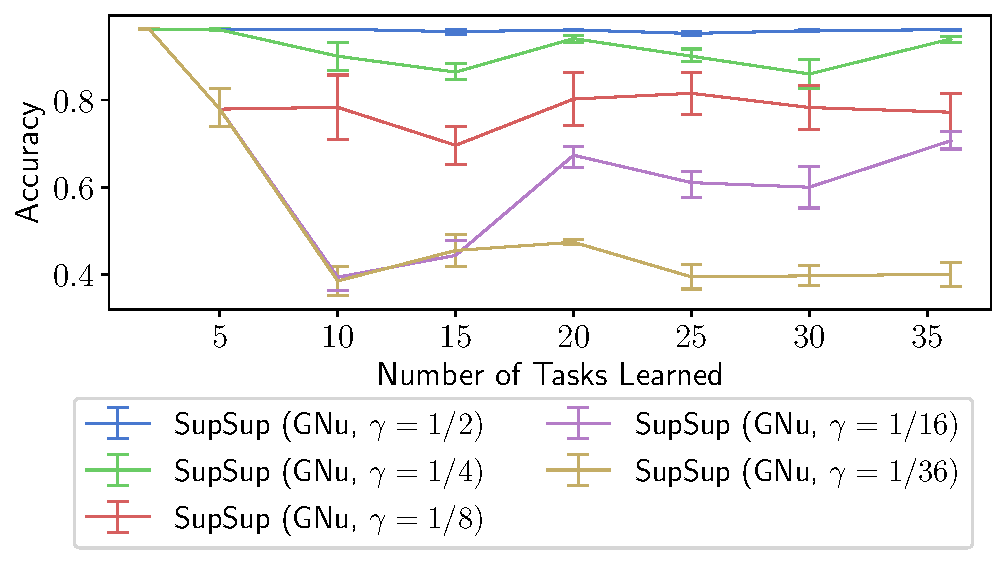
\includegraphics[scale=0.33]{rebuttal/rebut.pdf}
    \end{subfigure}
    \begin{subfigure}{0.3\textwidth}
    \centering
    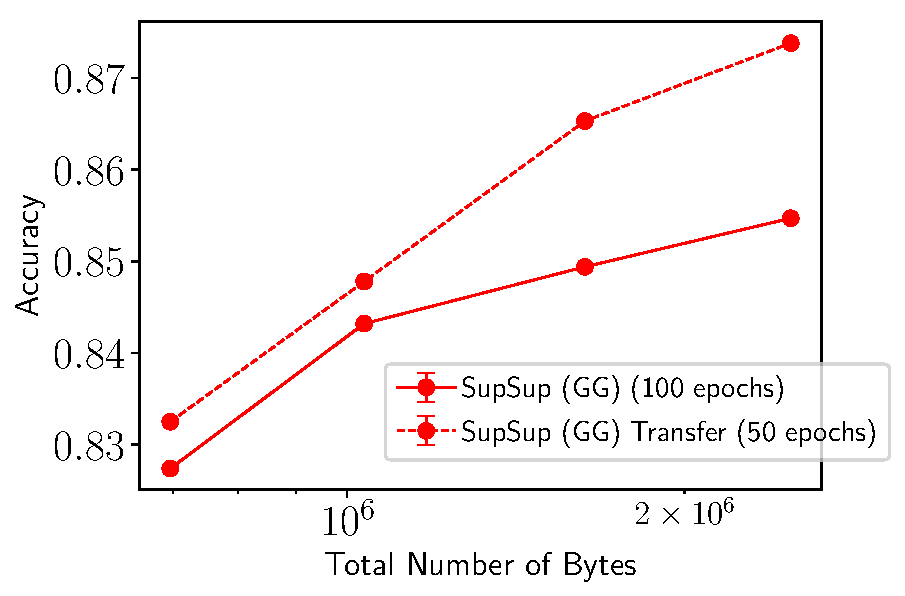
\includegraphics[scale=0.3]{rebuttal/estop.pdf}
    \end{subfigure}
    \begin{subfigure}{0.33\textwidth}
    \centering
    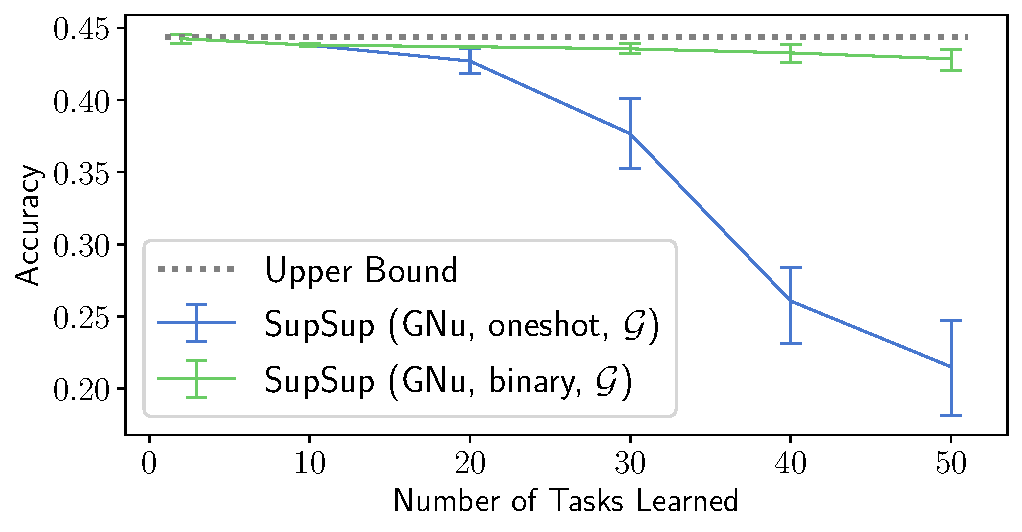
\includegraphics[scale=0.33]{rebuttal/cifarperm.pdf}
    \end{subfigure}
     \label{fig:rf}
    \caption{\textbf{(left)} Interpolating between the binary and one-shot algorithm with $\gamma$. \textbf{(center)} Transfer enables faster learning on SplitCIFAR. \textbf{(right)} One-shot vs. binary for permutations of CIFAR. Figures viewed best with zoom.}
    \vspace*{-1em}
\end{figure}

\noindent \textbf{\textcolor{cl6}{\textbullet}} $\rtwo$: We appreciate the suggestions, in particular to enhance the clarity of the figures which will improve the paper. 
For further comparisons please see the \textbf{Further Comparison in \casename{GNu}} section in $\rone$ above. %Although more challenging settings did not appear in earlier CL literature, or even [1,2], they are gaining traction. For example, \casename{GNu} is referred to as ``Class-IL'' in [3] and ``Class learning'' in [4] as we illustrate in Table 1 of the Related Work section. 
In reference to the comments concerning lack of novelty and lack of coverage of previous approaches we highlight $\rthree$'s comments: 1) \textit{Applying supermasks to a continual learning scenario is definitely novel, and of interest to the community} and 2) \textit{The paper has a lot of prior work to cover (CL, supermasks, batch ensembles) and is done correctly. Prior work is concise and clear.} The most similar approach to SupSup is [4] and they are limited to scenario \casename{GG} while requiring more storage.

\noindent \textbf{\textcolor{cl10}{\textbullet}} $\rthree$: We are grateful for a comprehensive and thoughtful review.
We complete variants of the two very useful experiments that you have suggested, and detail the results below.

\textbf{Forward transfer.} Thank you for highlighting the importance of transfer. We illustrate in Figure 1 \textbf{(center)} that our method for transfer (initializing each new mask with a running mean of previous masks) does enable faster learning (less epochs are required to reach a given accuracy). Training all tasks for 50 epochs with our transfer method provides a significant accuracy boost over training individually on all tasks for 100 epochs for SplitCIFAR.

\textbf{Towards more complex tasks.}  We illustrate in Figure 1 \textbf{(right)} that SupSup with the binary algorithm can sequentially learn 50 permutations of CIFAR pixels with minimal forgetting. As in the paper we use the FC-1024-1024 network and train on each task for 1000 iterations, and accordingly the upper bound accuracy is low. However, we are most interested in the deviation from the upper bound. We will update the introduction to better reflect the scope of the paper.

{\small
[1] Brian Cheung \textit{et al.}. Superposition of many models into one. NeurIPS 2019.

[2] Yeming Wen, Dustin Tran, and Jimmy Ba. Batchensemble: an alternative approach to efficient ensemble and lifelong learning. ICLR 2020.

[3] Gido M van de Ven and Andreas S Tolias. Three scenarios for continual learning.
arXiv, 2019.

[4] Arun Mallya, \textit{et al.}: Adapting a single network to
multiple tasks by learning to mask weights. ECCV, 2018. 
}
\end{document}
